\chapter{Modelagem de Processo de Negócio}
\label{cp:bpmn}

Para a elaboração dos modelos de processos de negócio, é relevante o conhecimento de todos os elementos envolvidos na execução de processos, tais como atores, clientes internos e externos, recursos e limitações; por meio dos quais é estabelecido um modelo que propicia um melhor entendimento, organização e representação, seja esta uma visão contextual abstrata ou com alto nível de detalhamento, conforme necessário. 

Tipicamente, a representação de um modelo de processos inclui ícones, que representam atividades, eventos, decisões, condições e outros elementos do processo \cite{brazil2011bpm}. Esses elementos podem conter informações sobre os relacionamentos entre eles e com o ambiente, bem como sobre o comportamento de cada elemento na cadeia de processos.

\section{\textit{Business Process Modeling and Notation}}

A especificação da notação BPMN foi elaborada e lançada em 2004 pelo Instituto de Gerenciamento de Processos de Negócio ou BPMI (\textit{Business Process Management Institute}), que realizou fusão ao Consórcio OMG. Posteriormente, a notação BPMN foi adotada pelo Consórcio OMG como o padrão para modelagem de processos. Após a padronização, foram lançadas algumas versões subsequentes, atualmente encontrando-se na versão 2.0 \cite{object2016business}.

Segundo \citeauthoronline{correia2015enhancing}~(\citeyear{correia2015enhancing}), \textit{Business Process Modeling and Notation} (BPMN) é atualmente a notação de modelagem de processos de negócio mais usada entre profissionais da área, devido a sua flexibilidade e abrangência. Consiste em uma tecnologia recente e pode ser utilizada por profissionais com diferentes níveis de conhecimento técnico. A formalização dos conceitos de modelagem de processos de negócio é baseada em um metamodelo construído a partir da linguagem \textit{Unified Modeling Language} (UML). 

A construção de processos de negócio através desta notação, utiliza um conjunto de padrões denominado ``metamodelo para definição de processos de negócio'' \cite{object2016business}. Nesse sentido, a especificação BPMN provê uma notação gráfica para representar processos de negócio por meio de um diagrama chamado ``diagrama de processo de negócio''. Esse diagrama é elaborado a partir de um conjunto de elementos gráficos que compõem diagramas simples de serem desenvolvidos e
compreendidos. 

\begin{figure}[!ht]
\centering
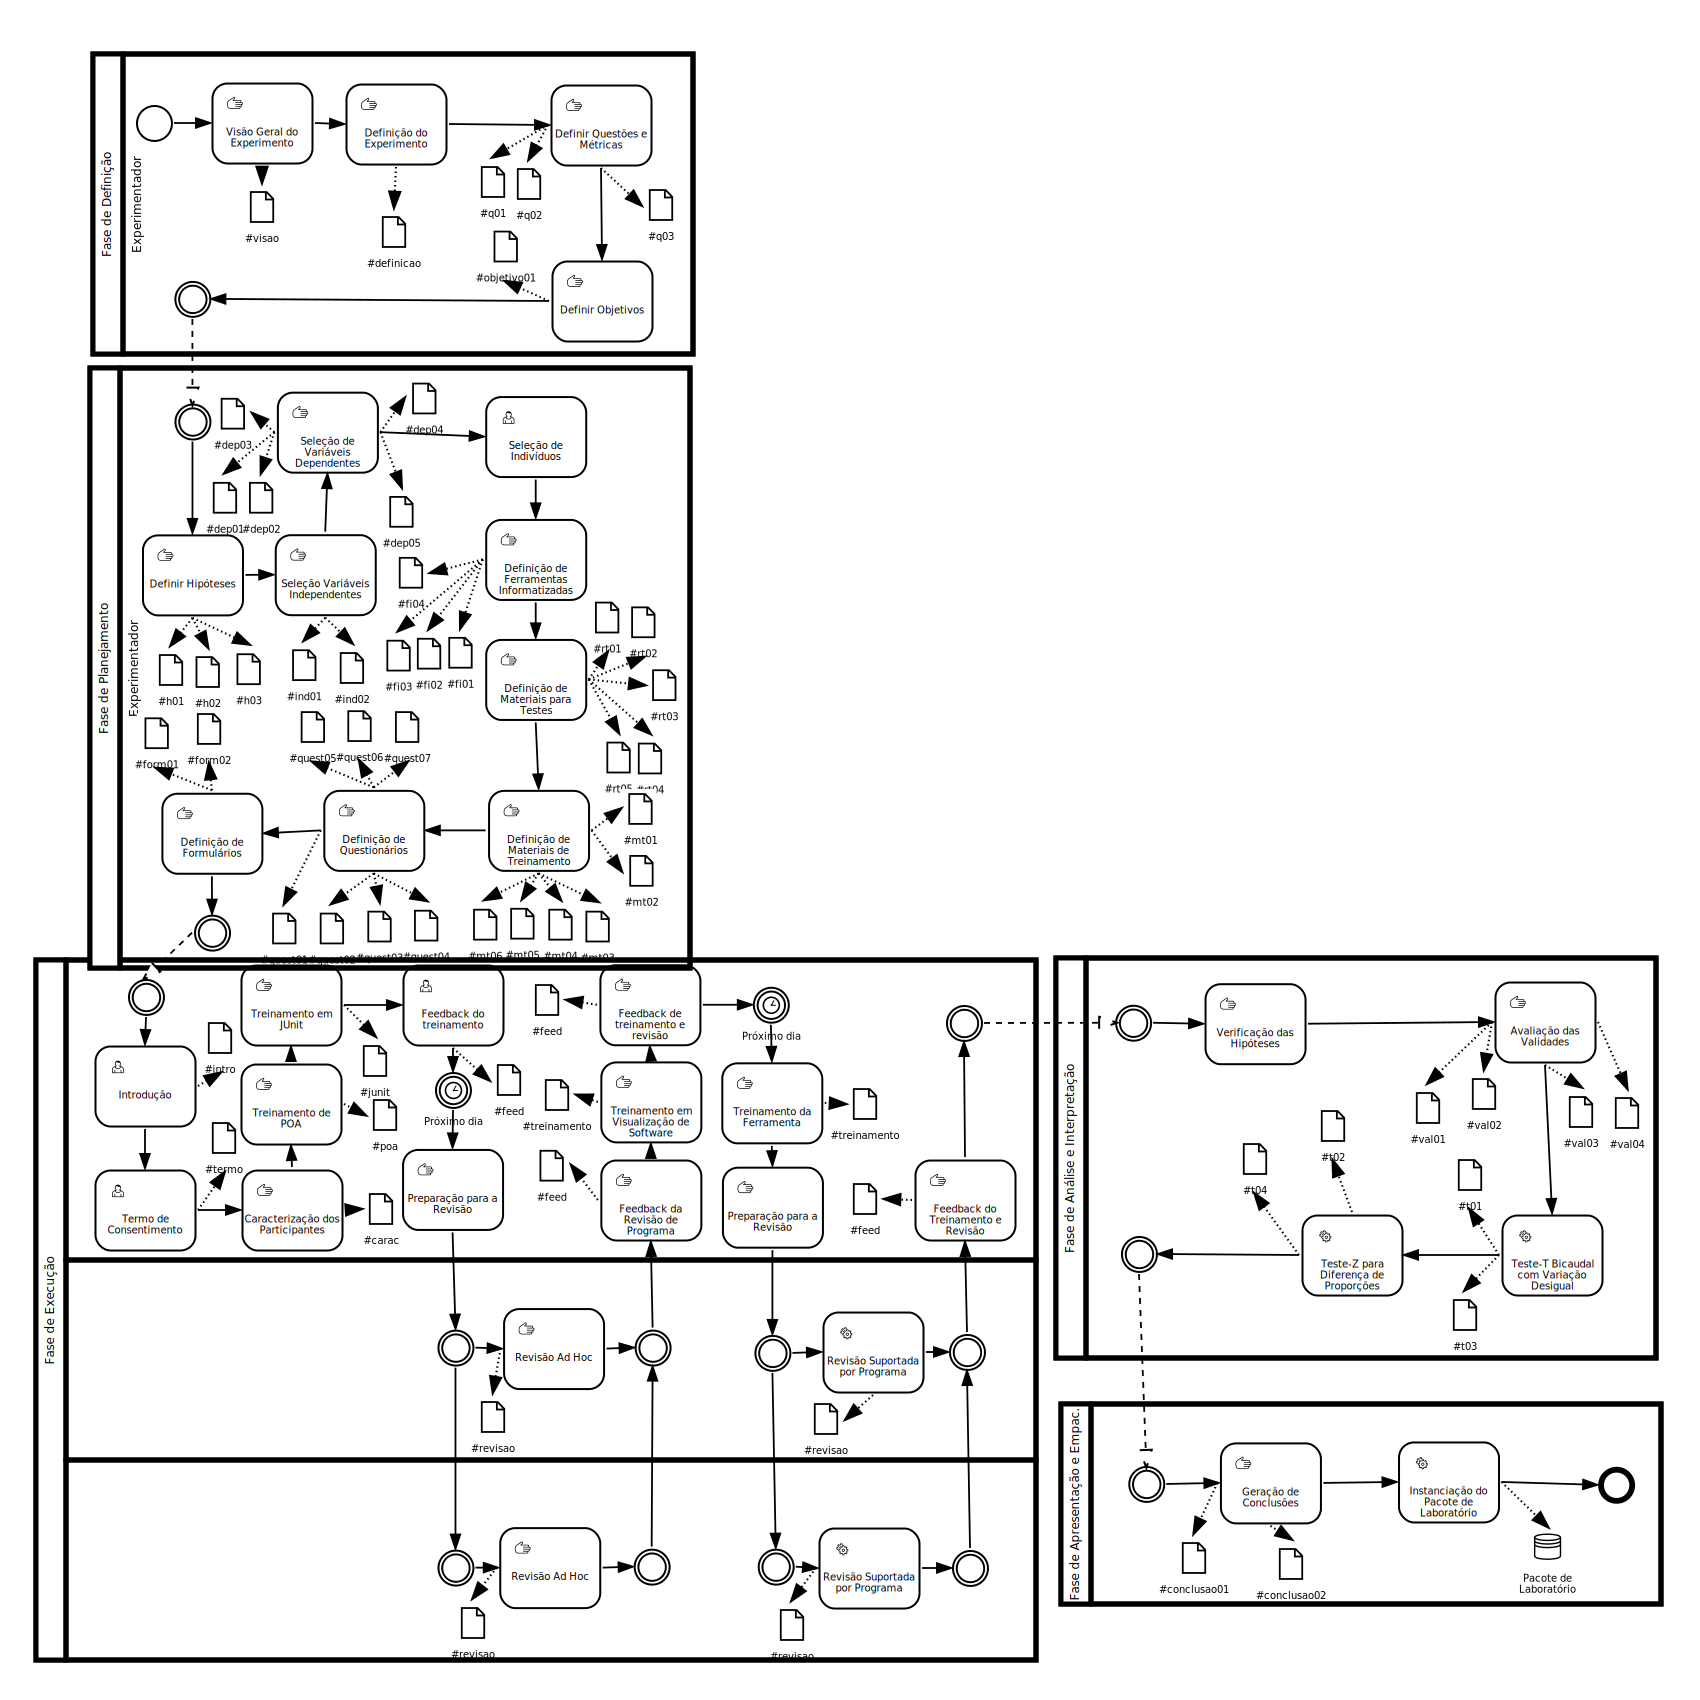
\includegraphics[scale=0.5]{images/diagrama.png}
\caption{Exemplo de diagrama BPMN – adaptado de \cite{Weske2012}.}
\label{diag}
\end{figure}

A Figura \ref{diag} apresenta, como exemplo, um simples diagrama de processo de negócio, através do qual é possível identificar a interação entre dois atores através da execução de atividades e trocas de mensagens, assim como, o uso de recursos como artefatos e repositórios de dados.

A especificação completa da atual versão define atributos que são agrupados em quatro categorias básicas de elementos: objetos de fluxo (\textit{Flow Objects}), objetos de conexão (\textit{Connecting Objects}), vias (\textit{Swimlanes}) e artefatos (\textit{Artifacts}). 
Na a Figura~\ref{elementos} há uma visão geral dos elementos da atual versão do BPMN.

\begin{figure}[!ht]
\centering
\includegraphics[scale=0.5]{images/elementos.png}
\caption{Conjunto de elementos que compõem a versão BPMN 2.0 \cite{object2016business}.}
\label{elementos}
\end{figure}

\section{Protocolos de experimentação usando BPM}

Compreender o projeto do experimento e revisar suas informações é fundamental não só para a execução do experimento, mas também para sua replicação. Diversos pesquisadores tem realizado projetos pilotos que ocasionam somente aumento de custos \cite{Kitchenham2008}. 

A utilização da notação de processo de negócio pode contribuir diretamente tanto na concepção quanto na execução do protocolo de estudo experimental. Primeiramente, devido à facilidade de compreensão do uso que compõem a respectiva notação, principalmente pelo fato de consistir em um padrão UML. Em segundo ponto, a utilização de pacotes de laboratório para o armazenamento das informações relativas aos protocolos realizados em cada experimento.

Através destes modelos de processo a seguir, é possível observar a sequência de execução das atividades, os fatores limitantes, tais como tempo, e também a estruturação de cada um dos processos e suas subdivisões.

Nas figuras \ref{selecao}, \ref{g1} e \ref{g2} são apresentados os diagramas de processo de negócio referentes ao protocolo de experimentação aplicado como parte do projeto de mestrado entitulado ``ModelUI$_{VIZ}$ - Uma proposta para representação de modelos de interface do usuário utilizando Visualização de Informação'', sob responsabilidade de Livia Cristina Gabos Martins, participante do Laboratório de Pesquisa em Engenharia de Software Aplicada -- LaPESA.

A representação do modelo de diagrama de processo de negócio também deve ser armazenado no pacote de laboratório, viabilizando o compartilhamento do protocolo juntamente com os dados referentes ao experimento, tais como hipóteses, variavéis dependentes e independentes.

%%%%%%%%%%%%%% selecao grupos
\begin{figure}[!ht]
\centering
\includegraphics[scale=0.7]{images/selecao.png}
\caption{Processo de atribuição de participantes aos grupos.}
\label{selecao}
\end{figure}


\begin{landscape}

%%%%%%%%%%%%%% grupo 01
\begin{figure}[!ht]
\centering
\includegraphics[scale=0.7]{images/grupo01.png}
\caption{Diagrama BPM referente às atividades dos participantes do primeiro grupo.}
\label{g1}
\end{figure}



%%%%%%%%%%%%%%% grupo 02
\begin{figure}[!ht]
\centering
\includegraphics[scale=0.7]{images/grupo02.png}
\caption{Diagrama BPM referente às atividades dos participantes do segundo grupo.}
\label{g2}
\end{figure}


\end{landscape}




